\chapter{Krachten, momenten, spanningne en rekken}

    \section{STATICA EN EVENWICHT VAN CONSTRUCTIES}

        \subsection{Types ondersteuningen}

            \begin{center}
                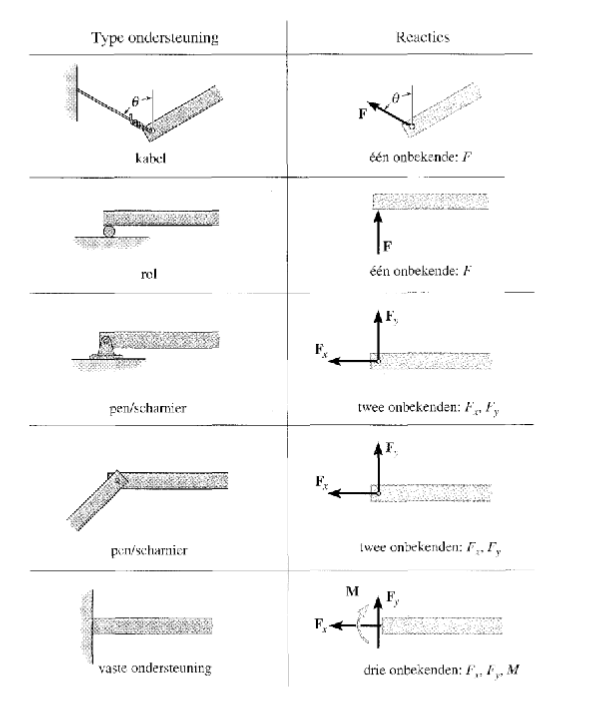
\includegraphics[scale=0.5]{ondersteuningen.png}
            \end{center}

        \subsection{Evenwicht van een constructie}

            \begin{align*}
                &\sum\mathbf{F} = 0\\
                &\sum\mathbf{M}_O = 0\\
            \end{align*}
    
    \section{INTUÏtIEF BEGRIP VAN SPANNINGEN EN REKKEN}

        \begin{align*}
            &\upsigma = \frac{F}{A_0}\\
            &\upvarepsilon = \frac{\Delta L}{L_0}\\
            &\upsigma = E\cdot \upvarepsilon
        \end{align*}

    \section{SPANNINGEN}
        
        \subsection{Definitie}

            De spanningsvector
            \begin{equation}
                \vec{\upphi}^{(n)} = \lim_{\Delta A \rightarrow 0} \frac{\Delta F}{\Delta A}
                \label{spanningsvector}
            \end{equation}
            De normaalspanning
            \begin{equation}
                \upsigma = \lim_{\Delta A \rightarrow 0} \frac{\Delta F_n}{\Delta A}
                \label{normaalspanning}
            \end{equation}
            De schuifspanning
            \begin{equation}
                \uptau = \lim_{\Delta A \rightarrow 0} \frac{\Delta F_t}{\Delta A}
                \label{schuifspanning}
            \end{equation}
            De spanningstensor
            \begin{equation}
                [\sigma] = \left[\begin{matrix}
                    \upsigma_{xx} & \uptau_{xy} & \uptau_{xz} \\
                    \uptau_{yx} & \upsigma_{yy} & \uptau_{yz} \\
                    \uptau_{zx} & \uptau_{zy} & \upsigma_{zz}
                \end{matrix}\right]
                \label{spanningstensor}
            \end{equation}

        \subsection{Verband tussen spanningsvector $\vec{\upphi}^{(n)}$ en spanningstensor $[\upsigma]$}
            
            Het verband tussen de spanningsvector en spanningstensor
            \begin{equation}
                \upsigma_{ij}\cdot n_i = \upphi_j^{(n)} \;\;\; (i,j=x,y,z)
                \label{spannigsvector_tensor}
            \end{equation}

        \subsection{Vergelijkingen van het evenwicht}

            De vergelijkingen van het evenwicht
            \begin{align}
                &\frac{\partial \upsigma_{xx}}{\partial x} + \frac{\partial \uptau_{yx}}{\partial y} + \frac{\partial \uptau_{zx}}{\partial z} + F_x = 0\nonumber\\
                &\frac{\partial \uptau_{xy}}{\partial x} + \frac{\partial \upsigma_{yy}}{\partial y} + \frac{\partial \uptau_{zy}}{\partial z} + F_y = 0\nonumber\\
                &\frac{\partial \uptau_{xz}}{\partial x} + \frac{\partial \uptau_{yz}}{\partial y} + \frac{\partial \upsigma_{zz}}{\partial z} + F_z = 0\nonumber\\
                \label{vergelijkingen_van_het_evenwicht}
            \end{align}
            Wet van de wederkerigheid der schuifspanningen
            \begin{align}
                &\uptau_{xy} = \uptau_{yx}\nonumber\\
                &\uptau_{xz} = \uptau_{zx}\nonumber\\
                &\uptau_{yz} = \uptau_{zy}\nonumber\\
            \end{align}

        \subsection{Transformatie van coördinaten en hoofdrichtingen}

            Transformatieregels
            \begin{equation}
                [\upsigma'] = [a]\cdot[\upsigma]\cdot[a]^{\top}
                \label{spanningstransformatie}
            \end{equation}
            met
            \begin{equation}
                a_{rk} = \vec{e}'_r\cdot\vec{e}_k \;\;\; r,k=x,y,z
                \label{Transformatiematrixelementen}
            \end{equation}
            Diagonaalsom van $[\upsigma]$
            \begin{equation}
                \Sigma_1 = \upsigma_{xx} + \upsigma_{yy} + \upsigma_{zz}
                \label{Diagonaalsom_sigma}
            \end{equation}
            Som van de hoofdminoren van $[\upsigma]$
            \begin{equation}
                \Sigma_2 = \upsigma_{xx}\upsigma_{yy} + \upsigma_{xx}\upsigma_{zz} + \upsigma_{yy}\upsigma_{zz} - \uptau_{xy}^2 - \uptau_{xz}^2 - \uptau_{yz}^2
                \label{Hoofdminoren_sigma}
            \end{equation}
            Determinant van $[\upsigma]$
            \begin{equation}
                \Sigma_3 = \upsigma_{xx}\upsigma_{yy}\upsigma_{zz} - \upsigma_{xx}\uptau_{yz}^2-\upsigma_{yy}\uptau_{xz}^2-\upsigma_{zz}\uptau_{xy}^2+2\uptau_{xy}\uptau_{xz}\uptau_{yz}
                \label{Determinant_sigma}
            \end{equation}

        \subsection{Kromlijnige coördinaten}
            
            \subsubsection{Cilindercoördinaten}

                De spanningstensor
                \begin{equation}
                    [\upsigma] = \left[\begin{matrix}
                        \upsigma_{rr} & \uptau_{x\theta} & \uptau_{rz} \\
                        \uptau_{r\theta} & \upsigma_{\theta \theta} & \uptau_{\theta z} \\
                        \uptau_{rz} & \uptau_{\theta z} & \upsigma_{zz}
                        \label{spanningstensor_cilinder}
                    \end{matrix}\right]
                \end{equation}
                De evenwichtsvergelijkingen
                \begin{align}
                    \frac{\partial \upsigma_{rr}}{\partial r} + \frac{\upsigma_{rr}-\upsigma_{\theta\theta}}{r} + \frac{1}{r}\frac{\partial \tau_{r\theta}}{\partial \theta} + \frac{\partial \uptau_{r\theta}}{\partial z} + F_r & = 0\nonumber\\
                    \frac{\partial \uptau_{r\theta}}{\partial r} + \frac{2\uptau_{r\theta}}{r} + \frac{1}{r}\frac{\partial \upsigma_{\theta\theta}}{\partial \theta}+\frac{\partial \uptau_{\theta z}}{\partial z}+F_{\theta} & = 0\nonumber\\
                    \frac{\partial \uptau_{rz}}{\partial r} + \frac{\uptau_{rz}}{r} + \frac{1}{r}\frac{\partial \uptau_{\theta z}}{\partial \theta}+\frac{\partial \upsigma_{zz}}{\partial z}+F_z & = 0\nonumber\\
                    \label{vergelijkingen_van_het_evenwicht_cilinder}
                \end{align}

            \subsubsection{Bolcoördinaten}
            De spanningstensor
            \begin{equation}
                [\upsigma] = \left[\begin{matrix}
                    \upsigma_{rr} & \uptau_{x\theta} & \uptau_{r\upphi} \\
                    \uptau_{r\theta} & \upsigma_{\theta \theta} & \uptau_{\theta\upphi} \\
                    \uptau_{r\upphi} & \uptau_{\theta\upphi} & \upsigma_{\upphi\upphi}
                    \label{spanningstensor_bol}
                \end{matrix}\right]
            \end{equation}
            De evenwichtsvergelijkingen
            \begin{align}
                \frac{\partial \upsigma_{rr}}{\partial r} + \frac{1}{r}\frac{\partial \tau_{r\theta}}{\partial \theta} + \frac{1}{r\sin\theta} + \frac{1}{r}\left(2\upsigma_{rr} + \uptau_{r\theta}\cot\theta-\upsigma_{\theta\theta}-\upsigma_{\upphi\upphi}\right) + F_r & = 0\nonumber\\
                \frac{\partial \uptau_{r\theta}}{\partial r} + \frac{1}{r}\frac{\partial \upsigma_{\theta\theta}}{\partial \theta} + +\frac{1}{r\sin\theta}\frac{\partial \uptau_{\theta\upphi}}{\upphi} + \frac{1}{r}\left(3\uptau_{r\theta} + \upsigma_{\theta\theta}\cot\theta-\upsigma_{\upphi\upphi}\cot\theta\right) + F_{\theta} & = 0\nonumber\\
                \frac{\partial \uptau_{r\upphi}}{\partial r} + \frac{1}{r}\frac{\partial \uptau_{\theta\upphi}}{\partial \theta} + \frac{1}{r\sin\theta}\frac{\partial \upsigma_{\upphi\upphi}}{\upphi} + \frac{1}{r}\left(3\uptau_{r\upphi} + 2\uptau_{\theta\upphi}\cot\theta\right)+ F_{\upphi} & = 0\nonumber\\
                \label{vergelijkingen_van_het_evenwicht_bol}
            \end{align}                

    \section{REKKEN}

        \subsection{Veralgemeende vervormingstoestand}

            Verband tussen rekken en verplaatsing
            \begin{align}
                \varepsilon_{xx} &= \frac{\partial u}{\partial x} \nonumber\\
                \varepsilon_{yy} &= \frac{\partial v}{\partial y} \nonumber\\
                \varepsilon_{zz} &= \frac{\partial w}{\partial z} \nonumber\\
                \upgamma_{xy} &= \frac{\partial v}{\partial x} + \frac{\partial u}{\partial y} \nonumber\\
                \upgamma_{xz} &= \frac{\partial w}{\partial x} + \frac{\partial u}{\partial z} \nonumber\\
                \upgamma_{yz} &= \frac{\partial w}{\partial y} + \frac{\partial v}{\partial z} \nonumber\\
                \label{verband_rekken_verplaatsing}
            \end{align}

        \subsection{Transformatie van coördinaten en hoofdrichtingen}    

            Transformatieregels
            \begin{equation}
                [\varepsilon'] = [a]\cdot[\varepsilon]\cdot[a]^{\top} \;\;\; \text{ met } a_{rk} = \vec{e}'_r\cdot\vec{e}_k
                \label{rektransformatie}
            \end{equation}
            De rekstensor
            \begin{equation}
                [\varepsilon] = \left[\begin{matrix}
                    \varepsilon_{xx} & \frac{1}{2}\upgamma_{xy} & \frac{1}{2}\upgamma_{xz} \\
                    \frac{1}{2}\upgamma_{xy} & \varepsilon_{yy} & \frac{1}{2}\upgamma_{yz} \\
                    \frac{1}{2}\upgamma_{xz} & \frac{1}{2}\upgamma_{yz} & \varepsilon_{zz}
                \end{matrix}\right] = \left[\begin{matrix}
                    \varepsilon_{xx} & \varepsilon_{xy} & \varepsilon_{xz} \\
                    \varepsilon_{xy} & \varepsilon_{yy} & \varepsilon_{yz} \\
                    \varepsilon_{xz} & \varepsilon_{yz} & \varepsilon_{zz}
                \end{matrix}\right]
                \label{rektensor}
            \end{equation}
            Diagonaalsom van $[\varepsilon]$
            \begin{equation}
                i_1 = \varepsilon_{xx} + \varepsilon_{yy} + \varepsilon_{zz}
                \label{Diagonaalsom_epsilon}
            \end{equation}
            Som van de hoofdminoren van $[\varepsilon]$
            \begin{equation}
                I_2 = \varepsilon_{xx}\varepsilon_{yy} + \varepsilon_{xx}\varepsilon_{zz} + \varepsilon_{yy}\varepsilon_{zz} - \varepsilon_{xy}^2 - \varepsilon_{xz}^2 - \varepsilon_{yz}^2
                \label{Hoofdminoren_epsilon}
            \end{equation}
            Determinant van $[\varepsilon]$
            \begin{equation}
                I_3 = \varepsilon_{xx}\varepsilon_{yy}\varepsilon_{zz} - \varepsilon_{xx}\varepsilon_{yz}^2-\varepsilon_{yy}\varepsilon_{xz}^2-\varepsilon_{zz}\varepsilon_{xy}^2+2\varepsilon_{xy}\varepsilon_{xz}\varepsilon_{yz}
                \label{Determinant_epsilon}
            \end{equation}
                
        \subsection{Compatibiliteitsvoorwaarden}

            \begin{align}
                \frac{\partial^2\varepsilon_{xx}}{\partial y\partial z} &= \frac{\partial}{\partial x} \left(\frac{\partial\varepsilon_{xz}}{\partial y} + \frac{\partial \varepsilon_{xy}}{\partial z} - \frac{\partial \varepsilon_{yz}}{\partial x}\right)\nonumber\\
                \frac{\partial^2\varepsilon_{yy}}{\partial x\partial z} &= \frac{\partial}{\partial y} \left(\frac{\partial\varepsilon_{xy}}{\partial z} + \frac{\partial \varepsilon_{yz}}{\partial x} - \frac{\partial \varepsilon_{xz}}{\partial y}\right)\nonumber\\
                \frac{\partial^2\varepsilon_{zz}}{\partial x\partial y} &= \frac{\partial}{\partial z} \left(\frac{\partial\varepsilon_{yz}}{\partial x} + \frac{\partial \varepsilon_{xz}}{\partial y} - \frac{\partial \varepsilon_{xy}}{\partial z}\right)\nonumber\\
                \frac{\partial^2\varepsilon_{xy}}{\partial x\partial y} &= \frac{1}{2} \left(\frac{\partial\varepsilon_{xx}}{\partial y^2} + \frac{\partial^2 \varepsilon_{yy}}{\partial x^2}\right)\nonumber\\
                \frac{\partial^2\varepsilon_{xz}}{\partial x\partial z} &= \frac{1}{2} \left(\frac{\partial\varepsilon_{zz}}{\partial x^2} + \frac{\partial^2 \varepsilon_{xx}}{\partial z^2}\right)\nonumber\\
                \frac{\partial^2\varepsilon_{yz}}{\partial y\partial z} &= \frac{1}{2} \left(\frac{\partial\varepsilon_{yy}}{\partial z^2} + \frac{\partial^2 \varepsilon_{zz}}{\partial y^2}\right)\nonumber\\
                \label{compatibiliteitsvoorwarden}
            \end{align}

       \subsection{Kromlijnige coördinaten}     

            \subsubsection{Cilindercoördinaten}

                \begin{equation}
                    [\varepsilon] = \left[\begin{matrix}
                        \varepsilon_{rr} & \frac{1}{2}\upgamma_{r\theta} & \frac{1}{2}\upgamma_{rz} \\
                        \frac{1}{2}\upgamma_{r\theta} & \varepsilon_{\theta\theta} & \frac{1}{2}\upgamma_{\theta z} \\
                        \frac{1}{2}\upgamma_{rz} & \frac{1}{2}\upgamma_{\theta z} & \varepsilon_{zz}
                    \end{matrix}\right] = \left[\begin{matrix}
                        \frac{\partial u_r}{\partial r} & \frac{1}{2}\left(\frac{1}{r}\frac{\partial u_r}{\partial \theta} + \frac{\partial u_\theta}{\partial r} - \frac{u_{\theta}}{r}\right) & \frac{1}{2}\left(\frac{\partial u_r}{\partial r} + \frac{\partial u_z}{\partial r}\right)\\
                        \frac{1}{2}\left(\frac{1}{r}\frac{\partial u_r}{\partial \theta} + \frac{\partial u_{\theta}}{\partial r} - \frac{u_{\theta}}{r}\right) & \frac{u_r}{r} + \frac{1}{r}\frac{\partial u_{\theta}}{\partial \theta} & \frac{1}{2}\left(\frac{\partial u_{\theta}}{\partial z} + \frac{1}{r}\frac{\partial u_z}{\partial \theta}\right)\\
                        \frac{1}{2}\left(\frac{\partial u_r}{\partial z} + \frac{\partial u_z}{\partial r}\right) & \frac{1}{2}\left(\frac{\partial u_{\theta}}{\partial z} + \frac{1}{r}\frac{\partial u_z}{\partial \theta}\right) & \frac{\partial u_z}{\partial z}
                    \end{matrix}\right]
                    \label{rektensor_cilinder}
                \end{equation}

            \subsubsection{Bolcoördinaten}
            
                \begin{align}
                    [\varepsilon] &= \left[\begin{matrix}
                        \varepsilon_{rr} & \frac{1}{2}\upgamma_{r\theta} & \frac{1}{2}\upgamma_{rz} \\
                        \frac{1}{2}\upgamma_{r\theta} & \varepsilon_{\theta\theta} & \frac{1}{2}\upgamma_{\theta \upphi} \\
                        \frac{1}{2}\upgamma_{r\upphi} & \frac{1}{2}\upgamma_{\theta \upphi} & \varepsilon_{\upphi\upphi}
                    \end{matrix}\right] \nonumber\\
                    &= \left[\begin{matrix} 
                        \frac{\partial u_r}{\partial r} & \frac{1}{2}\left(\frac{1}{r}\frac{\partial u_r}{\partial \theta} + \frac{\partial u_{\theta}}{\partial r} - \frac{u_{\theta}}{r}\right) & \frac{1}{2}\left(\frac{1}{r\sin\theta}\frac{\partial u_r}{\partial \upphi} + \frac{\partial u_{\upphi}}{\partial r} - \frac{u_{\upphi}}{r}\right)\\
                        \frac{1}{2}\left(\frac{1}{r}\frac{\partial u_r}{\partial \theta} + \frac{\partial u_{\theta}}{\partial r} - \frac{u_{\theta}}{r}\right) & \frac{u_r}{r} + \frac{1}{r}\frac{\partial u_{\theta}}{\partial \theta} & \frac{1}{2}\left(\frac{1}{r\sin\theta}\frac{\partial u_{\theta}}{\partial \upphi} + \frac{1}{r}\frac{\partial u_{\upphi}}{\partial \theta} - \frac{u_{\upphi}}{r}\cot\theta\right)\\
                        \frac{1}{2}\left(\frac{1}{r\sin\theta}\frac{\partial u_r}{\partial \upphi} + \frac{\partial u_{\upphi}}{\partial r} - \frac{u_{\upphi}}{r}\right) & \frac{1}{2}\left(\frac{1}{r\sin\theta}\frac{\partial u_{\theta}}{\partial \upphi} + \frac{1}{r}\frac{\partial u_{\upphi}}{\partial \theta} - \frac{u_{\upphi}}{r}\cot\theta\right) & \frac{1}{r\sin\theta} + \frac{u_r}{r} + \frac{u_{\theta}}{r}\cot\theta
                    \end{matrix}\right] \nonumber
                    \label{rektensor_bol}
                \end{align}
        
        %\subsection{Eindige vervormingen en rekken}   % Rekken van Green: buiten het bestek van deze cursus

    \section{LINEAIR ELASTISCH MATERIAALGEDRAG}

        \subsection{Wet van Hooke}
            
            Wet van Hooke
            \begin{align}
                \varepsilon_{xx} &= \frac{1}{E}\left[\upsigma_{xx} - \upnu\left(\upsigma_{yy}+\upsigma_{zz}\right)\right]\nonumber\\
                \varepsilon_{yy} &= \frac{1}{E}\left[\upsigma_{yy} - \upnu\left(\upsigma_{xx}+\upsigma_{zz}\right)\right]\nonumber\\
                \varepsilon_{zz} &= \frac{1}{E}\left[\upsigma_{zz} - \upnu\left(\upsigma_{xx}+\upsigma_{yy}\right)\right]\nonumber\\
                \upgamma_{xy} &= \frac{\uptau_{xy}}{G}\nonumber\\
                \upgamma_{xz} &= \frac{\uptau_{xz}}{G}\nonumber\\
                \upgamma_{yz} &= \frac{\uptau_{yz}}{G}\nonumber\\
            \end{align}
            Geïnverteerde wet van Hooke
            \begin{align}
                \upsigma_{xx} &= \frac{E}{(1+\upnu)(1-2\upnu)}\left[(1-\upnu)\varepsilon_{xx}+\upnu\left(\varepsilon_{yy}+\varepsilon_{zz}\right)\right]\nonumber\\
                \upsigma_{yy} &= \frac{E}{(1+\upnu)(1-2\upnu)}\left[(1-\upnu)\varepsilon_{yy}+\upnu\left(\varepsilon_{xx}+\varepsilon_{zz}\right)\right]\nonumber\\
                \upsigma_{zz} &= \frac{E}{(1+\upnu)(1-2\upnu)}\left[(1-\upnu)\varepsilon_{zz}+\upnu\left(\varepsilon_{xx}+\varepsilon_{yy}\right)\right]\nonumber\\
                \uptau_{xy} &= G\upgamma_{xy}\nonumber\\
                \uptau_{xz} &= G\upgamma_{xz}\nonumber\\
                \uptau_{yz} &= G\upgamma_{yz}\nonumber\\
                \label{Wet_van_Hooke_inv}
            \end{align}
        
        \subsection{Bijzondere belastingsgevallen}

            \subsubsection{Zuivere rek}

                (x-as volgens trekrichting)
                \begin{equation}
                    [\upsigma] = \left[\begin{matrix}
                        \upsigma_{xx} & 0 & 0 \\
                        0 & 0 & 0 \\
                        0 & 0 & 0
                    \end{matrix}\right]
                \end{equation}
            
            \subsubsection{Zuivere afschuiving}
                
                (x-as volgens trekrichting)
                \begin{equation}
                    [\upsigma] = \left[\begin{matrix}
                        0 & 0 & \uptau_{xz} \\
                        0 & 0 & 0 \\
                        \uptau_{xz} & 0 & 0
                    \end{matrix}\right]
                \end{equation}
            
            \subsubsection{Hydrostatische belasting}

                \begin{equation}
                    [\upsigma] = \left[\begin{matrix}
                        \upsigma_{xx} & 0 & 0 \\
                        0 & \upsigma_{yy} & 0 \\
                        0 & 0 & \upsigma_{zz}
                    \end{matrix}\right] = \left[\begin{matrix}
                        -|p| & 0 & 0 \\
                        0 & -|p| & 0 \\
                        0 & 0 & -|p|
                    \end{matrix}\right]
                \end{equation}
                
            \subsubsection{Torsie of wringing}

                (x-as in de langsrichting)
                \begin{equation}
                    [\upsigma] = \left[\begin{matrix}
                        0 & \uptau_{xy} & \uptau_{xz} \\
                        \uptau_{xy} & 0 & 0 \\
                        \uptau_{xz} & 0 & 0
                    \end{matrix}\right]
                \end{equation}
                in polaire coördinaten
                \begin{equation}
                    [\upsigma] = \left[\begin{matrix}
                        0 & 0 & 0 \\
                        0 & 0 & \uptau_{\theta z} \\
                        0 & \uptau_{\theta z} & 0
                    \end{matrix}\right]
                \end{equation}
            
            \subsection{Relaties tussen de elastische constanten}
                
                \subsubsection{Verband tussen $E$, $\upnu$ en $G$}

                    \begin{equation}
                        G=\frac{E}{2(1+\upnu)}
                    \end{equation}

            \subsubsection{Volumeverandering en compressiemodulus}

                Volumerek of dilatatie
                \begin{equation}
                    \varepsilon_{\text{vol}} = \frac{\Delta V}{dV} = \varepsilon_{xx} + \varepsilon_{yy} + \varepsilon_{zz}
                \end{equation}
                Compressiemodulus of volume-elasticiteitsmodulus
                \begin{equation}
                    K = \frac{-|p|}{\frac{\Delta V}{dv}} = \frac{E}{3(1-2\upnu)}, \;\;\; \upnu \frac{1}{2}
                \end{equation}

        \subsection{Kromlijnige coördinaten}
            
            Cilindercoördinaten
            \begin{align}
                \varepsilon_{rr} &= \frac{1}{E}\left[\upsigma_{xx} - \upnu\left(\upsigma_{\theta\theta}+\upsigma_{zz}\right)\right]\nonumber\\
                \varepsilon_{\theta\theta} &= \frac{1}{E}\left[\upsigma_{\theta\theta} - \upnu\left(\upsigma_{xx}+\upsigma_{zz}\right)\right]\nonumber\\
                \varepsilon_{zz} &= \frac{1}{E}\left[\upsigma_{zz} - \upnu\left(\upsigma_{xx}+\upsigma_{\theta\theta}\right)\right]\nonumber\\
                \upgamma_{x\theta} &= \frac{\uptau_{x\theta}}{G}\nonumber\\
                \upgamma_{xz} &= \frac{\uptau_{rz}}{G}\nonumber\\
                \upgamma_{\theta z} &= \frac{\uptau_{\theta z}}{G}\nonumber\\
            \end{align}

    \section{OPLOSSING VAN HET LINEAIR ELASTISCH PROBLEEM}

        Gebruik \emph{vergelijkingen van het evenwicht}, \emph{vergelijkingen tussen rek en verplaatsing} en de wet van Hooke samen met randvoorwaarden om het linear statisch probleem op te lossen.

    \section{THERMISCHE SPANNINGEN}

        \subsection{Vergelijkingen}

            \begin{align}
                \varepsilon_{xx} &= \frac{1}{E}\left[\upsigma_{xx} - \upnu\left(\upsigma_{yy}+\upsigma_{zz}\right)\right] + \alpha T\nonumber\\
                \varepsilon_{yy} &= \frac{1}{E}\left[\upsigma_{yy} - \upnu\left(\upsigma_{xx}+\upsigma_{zz}\right)\right] + \alpha T\nonumber\\
                \varepsilon_{zz} &= \frac{1}{E}\left[\upsigma_{zz} - \upnu\left(\upsigma_{xx}+\upsigma_{yy}\right)\right] + \alpha T\nonumber\\
                \upgamma_{xy} &= \frac{\uptau_{xy}}{G}\nonumber\\
                \upgamma_{xz} &= \frac{\uptau_{xz}}{G}\nonumber\\
                \upgamma_{yz} &= \frac{\uptau_{yz}}{G}\nonumber\\
            \end{align}
            Geïnverteerd
            \begin{align}
                \upsigma_{xx} &= \frac{E}{(1+\upnu)(1-2\upnu)}\left[(1-\upnu)\varepsilon_{xx}+\upnu\left(\varepsilon_{yy}+\varepsilon_{zz}\right)\right] - \frac{E}{1-2\upnu}\alpha T\nonumber\\
                \upsigma_{yy} &= \frac{E}{(1+\upnu)(1-2\upnu)}\left[(1-\upnu)\varepsilon_{yy}+\upnu\left(\varepsilon_{xx}+\varepsilon_{zz}\right)\right] - \frac{E}{1-2\upnu}\alpha T\nonumber\\
                \upsigma_{zz} &= \frac{E}{(1+\upnu)(1-2\upnu)}\left[(1-\upnu)\varepsilon_{zz}+\upnu\left(\varepsilon_{xx}+\varepsilon_{yy}\right)\right] - \frac{E}{1-2\upnu}\alpha T\nonumber\\
                \uptau_{xy} &= G\upgamma_{xy}\nonumber\\
                \uptau_{xz} &= G\upgamma_{xz}\nonumber\\
                \uptau_{yz} &= G\upgamma_{yz}\nonumber\\
            \end{align}

    \section{ARBEID EN ELASTISCHE ENERGIE}

        \subsection{Arbeid van een kracht}

            Verichte arbeid
            \begin{equation}
                dU_{\text{uitw}} = F\cdot dx
            \end{equation}
            Totale arbeid over afstand x
            \begin{equation}
                U_{\text{uitw}} = \int^x_0F(x)\cdot dx
            \end{equation}

        \subsection{Arbeid van een moment}

            Verichte arbeid
            \begin{equation}
                dU_{\text{uitw}}=M\cdot d\theta
            \end{equation}
            Totale arbeid over hoekverdraaiing
            \begin{equation}
                U_{\text{uitw}} = \int^{\theta}_0M(\theta)\cdot\theta
            \end{equation}

        \subsection{Wet van behoud van mechanishce energie}

            \begin{equation}
                U_{\text{uitw}} = U_{\text{inw}}
            \end{equation}
                


                
        

